%%%%%%%%%%%%%%%%%%%%%%%%%%%%%%%%%%%%%%%%%
%
% (c) 2018 by Jennifer Laaser
%
% This work is licensed under the Creative Commons Attribution-NonCommercial-ShareAlike 4.0 International License. To view a copy of this license, visit http://creativecommons.org/licenses/by-nc-sa/4.0/ or send a letter to Creative Commons, PO Box 1866, Mountain View, CA 94042, USA.
%
% The current source for these materials is accessible on Github: https://github.com/jlaaser/quantum-exercises
%
%%%%%%%%%%%%%%%%%%%%%%%%%%%%%%%%%%%%%%%%%

\section*{Wavepackets\sectionmark{Exercise: Wavepackets}}

\begin{questions}
\question Activity time!  Get everyone in your group to stand up and stand shoulder-to-shoulder in a straight line.  You may go out in the hallway if you need more room.

	\begin{parts}
		\part Have everyone walk forward for 5 seconds.  Try to walk at as close to the same speed as possible.  Mark each person's initial and final positions on the following axis:

	\vspace{0.2in}
	\centerline{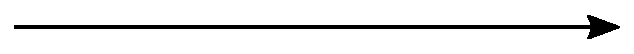
\includegraphics[width=0.6\textwidth]{includes/wavepackets-FIGURES/long-arrow.pdf}}
	\vspace{0.2in} 
		
		\part Go back to your starting line.  Have everyone walk forward for 5 seconds again, but this time, designate at least one person as a ``fast'' walker and one as a ``slow'' walker.  Mark each person's initial and final positions on the following axis:

	\vspace{0.2in}
	\centerline{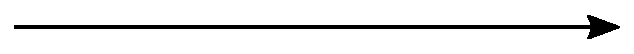
\includegraphics[width=0.6\textwidth]{includes/wavepackets-FIGURES/long-arrow.pdf}}
	\vspace{0.2in} 
		
		\part In which of these two ``simulations'' was the uncertainty in your momentum higher?  How was it reflected in your final position distribution?
			\begin{solution}[1.5in]
			\end{solution}
	\end{parts}

\question Consider a Gaussian wavepacket traveling to the right. At $t=0$, its probability distribution might look like this:

	\vspace{0.1in}
	\centerline{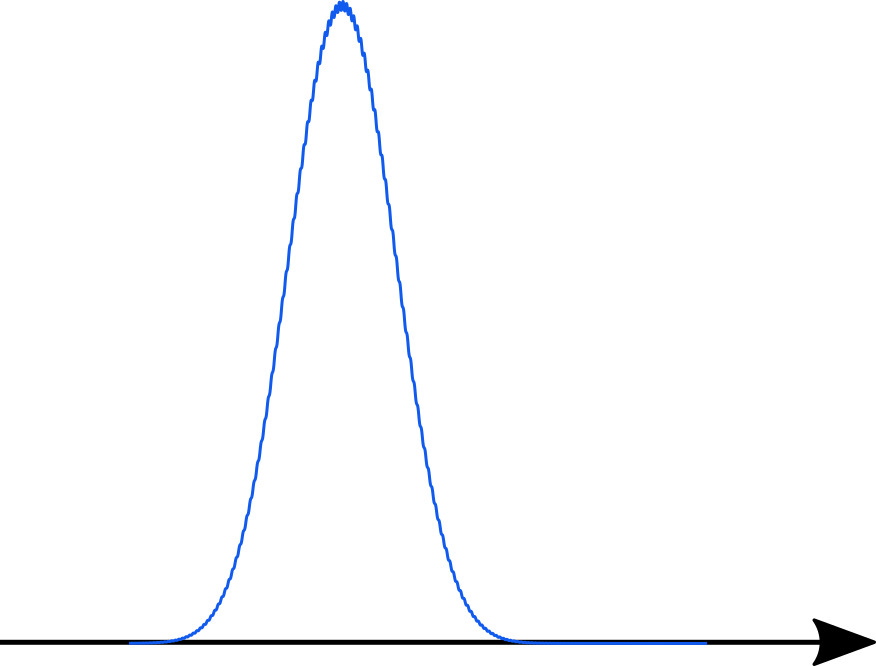
\includegraphics[width=0.35\textwidth]{includes/wavepackets-FIGURES/gaussian.jpg}}
	\vspace{0.1in} 
 
	\begin{parts}
		\part Based on the simulation you just did, what feature of this plot (if any) do you think gives you information about the uncertainty in the particle's position? Mark it on the plot.

		\part Similarly, what feature of this plot (if any) gives you information about the uncertainty in the particle's momentum?  Mark it on the plot.
	\end{parts}
	
	\contdnewpg

\question The following plots show the propagation of two different wavepackets:

      	\vspace{0.2in}
	\begin{minipage}{0.5\textwidth}
	\centerline{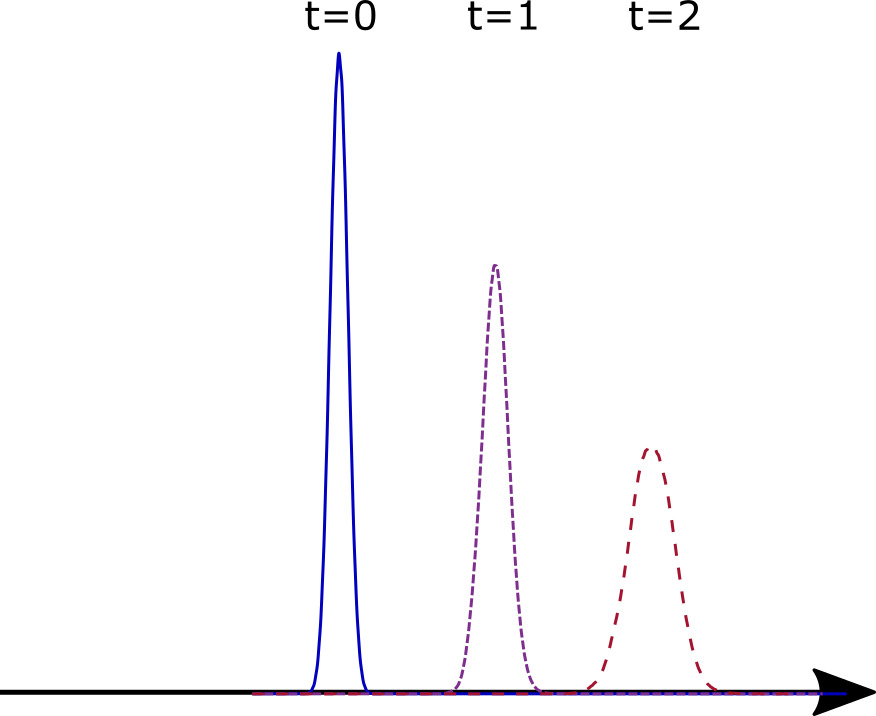
\includegraphics[width=0.8\textwidth]{includes/wavepackets-FIGURES/prop1.jpg}}
	\end{minipage}
	\begin{minipage}{0.5\textwidth}
	\centerline{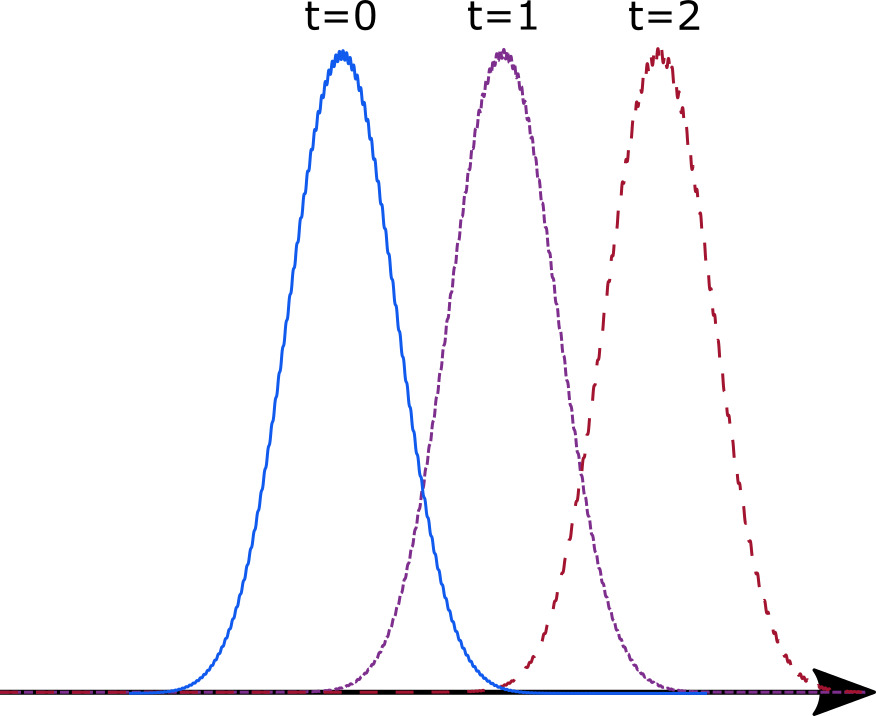
\includegraphics[width=0.8\textwidth]{includes/wavepackets-FIGURES/prop2.jpg}}
	\end{minipage}
	\vspace{0.1in}

\begin{parts}
\part Which wavepacket has the larger uncertainty in the position, and which has the larger uncertainty in the momentum?

	\begin{solution}[1.5in]
	\end{solution}

\part Explain how your observations relate to the uncertainty principle.
\end{parts}
	

\end{questions}
